% $Id: patches.tex 5703 2017-10-31 03:07:37Z mskala $

%
% MSK 007 patch ideas
% Copyright (C) 2017  Matthew Skala
%
% This program is free software: you can redistribute it and/or modify
% it under the terms of the GNU General Public License as published by
% the Free Software Foundation, version 3.
%
% This program is distributed in the hope that it will be useful,
% but WITHOUT ANY WARRANTY; without even the implied warranty of
% MERCHANTABILITY or FITNESS FOR A PARTICULAR PURPOSE.  See the
% GNU General Public License for more details.
%
% You should have received a copy of the GNU General Public License
% along with this program.  If not, see <http://www.gnu.org/licenses/>.
%
% Matthew Skala
% https://northcoastsynthesis.com/
% mskala@northcoastsynthesis.com
%

\chapter{Patch ideas}

Here's a basic subtractive synthesis patch:  pitch CV from the MIDI
interface connects to the V/octave inputs on a sawtooth oscillator and the
MSK~007, while the gate CV drives and ADSR envelope which controls the
built-in VCA on the MSK~007 (VCA mode switch set to ``output'').

\nopagebreak\noindent
{\hspace*{\fill}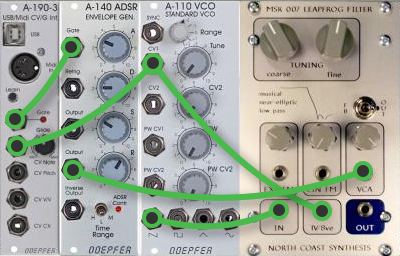
\includegraphics[scale=0.6]{patch1.png}\hspace*{\fill}\par} 

In a more elaborate subtractive synthesis patch, two ADSR envelopes drive
the amplitude and filter cutoff separately, with an external VCA which frees
the MSK~007's built-in VCA to provide feedback.

\nopagebreak\noindent
{\hspace*{\fill}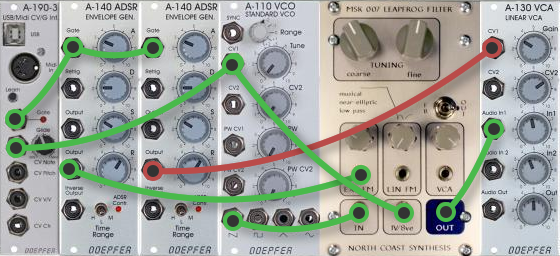
\includegraphics[scale=0.45]{patch2.png}\hspace*{\fill}\par} 

Deluxe subtractive synthesis patch demonstrating the use of the MSK~007 with
other North Coast Synthesis modules: the pitch CV goes through an MSK~008
Octave Switch (normalled to both channels) to provide separate manual octave
switching up and down for the VCO and the filter.  A sine wave from the
MSK~010 controls linear frequency modulation of the filter cutoff for a
unique effect.

\nopagebreak\noindent
{\hspace*{\fill}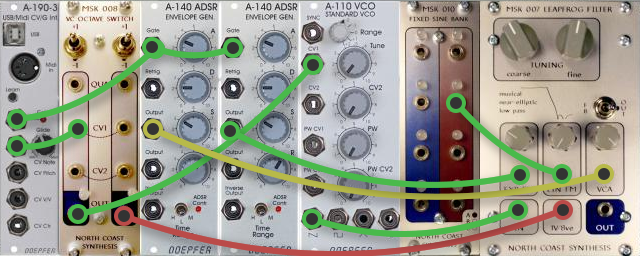
\includegraphics[scale=0.45]{patch3.png}\hspace*{\fill}\par} 

\pagebreak

The MSK~007 can be a minimal synth voice all by itself, using the
gate input to control the VCA in feedback mode to switch oscillation on and
off.  A MIDI interface is shown, but any CV-gate controller would work.

\nopagebreak\noindent
{\hspace*{\fill}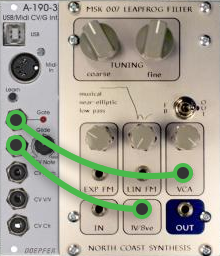
\includegraphics[scale=0.6]{patch4.png}\hspace*{\fill}\par} 

An envelope generator set up to create a spike (fast attack and decay,
zero sustain level) can ``ping'' the filter when fed into the audio input. 
Set the VCA to feedback mode and adjust the level to the point where it
almost, but not quite, sustains oscillation.

\nopagebreak\noindent
{\hspace*{\fill}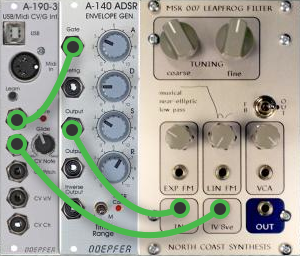
\includegraphics[scale=0.6]{patch5.png}\hspace*{\fill}\par}

Pinging with a noise burst instead of just a voltage spike produces a
different sound with some extra grit in the attack.

\nopagebreak\noindent
{\hspace*{\fill}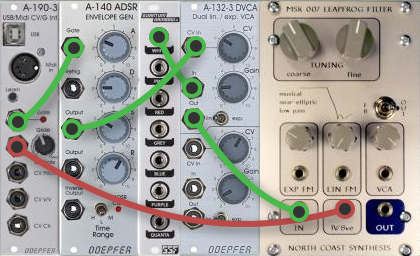
\includegraphics[scale=0.6]{patch6.png}\hspace*{\fill}\par} 

\pagebreak

The MSK~007 can take inputs all the way down to DC, so
with the cutoff frequency very low (at or near its minimum) it can process
control voltages as
an unusual kind of slew rate limiter, with a bit of bounce or overshoot on
rapidly-changing inputs (especially in feedback mode).  The gain through the
filter is not easy to adjust to precisely unity, so you might not want to
use this for critical melodic material; but with a square wave LFO input, as
shown, it puts an interesting twist on the control waveform for generating
a drone texture.

\nopagebreak\noindent
{\hspace*{\fill}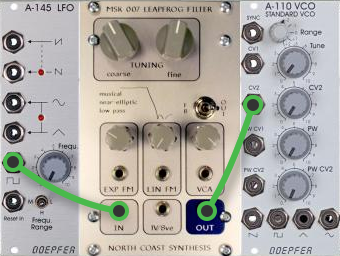
\includegraphics[scale=0.6]{patch7.png}\hspace*{\fill}\par} 

Doepfer's A-188-1 bucket brigade module does not include an output filter,
so at low clock rates the clock will be audible unless you filter it out
externally.  The MSK~007 is especially well-suited for that because of its
low cutoff.  With the MSK~007 tuned to cut off at the Nyquist frequency
(half the BBD's clock frequency), it will cleanly eliminate both clock and
alias signals.

\nopagebreak\noindent
{\hspace*{\fill}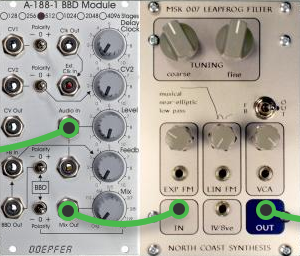
\includegraphics[scale=0.6]{patch8.png}\hspace*{\fill}\par} 

Spectral inversion is another use for a sharp low-pass filter.  Tune the
sine wave VCO (here used as a \emph{local oscillator}) to generate a carrier
a little above the highest frequency in the input.  Ring-modulate
(four-quadrant multiply) the input with the carrier.  That produces two
frequency bands: upper sideband consisting of the input shifted up by the
carrier frequency, and lower sideband consisting of all the input
frequencies subtracted from the carrier frequency.  The MSK~007
removes the upper sideband and any carrier feedthrough.

Spectral inversion is an interesting effect in itself, but you can also use
two copies of this patch (two MSK~007 modules, two oscillators,
and two channels of four-quadrant multiplication) with slightly
different carrier frequencies, to serve as a frequency shifter.

\nopagebreak\noindent
{\hspace*{\fill}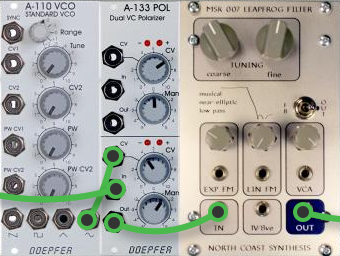
\includegraphics[scale=0.6]{patch9.png}\hspace*{\fill}\par} 
